\documentclass[../algebraIII_notes.tex]{subfiles}
\begin{document}
\section{Aula 16 - 09 de Junho, 2026}
\subsection{Motivações}
\begin{itemize}
	\item Extensões Ciclotômicas
\end{itemize}
\subsection{Extensões Ciclotômicas}
Um fato geral que usaremos hoje é que, para qualquer \(f(x)\in F[x]\), vale que ele é irredutível se, e somente se, \(f(x+1)\) também for.
\begin{exr}
	Cheque o fato geral acima.
\end{exr}
Como
\[
	C_{p}(x) = \frac{x^{p}-1}{(x-1)},
\]
temos
\[
	C_{p}(x+1) = \frac{(x+1)^{p}-1}{x} = x^{p-1} + \binom{p}{p-1}x^{p-2}+\dotsc +\binom{p}{3}x^{2}+\binom{p}{2}x + \binom{p}{1}.
\]
Em geral, para n qualquer, podemos considerar
\[
	\frac{\mathbb{Q}[x]}{(C_{n}(x))} \eqqcolon \mathbb{Q}(\zeta_{n}).
\]
\begin{def*}
	Chamamos o corpo \(\mathbb{Q}(\zeta_{n})\) de \textbf{n-ésimo corpo ciclotômico}. \(\square\)
\end{def*}
Uma propriedade interessante é que o grau de extensão de \(\mathbb{Q}(\zeta_{n})\) sobre \(\mathbb{Q}\) é dado pela função totiente de Euler de n.
\begin{lemma*}
	O corpo \(\mathbb{Q}(\zeta_{n})\) é um corpo de decomposição de \(x^{n}-1\).
\end{lemma*}
\begin{exr}
	Prove o lema enunciado.
\end{exr}
\begin{crl*}
	A extensão \(\mathbb{Q}(\zeta_{n})/\mathbb{Q}\) é Galois.
\end{crl*}
\begin{proof*}
	Basta notar que
	\[
		\frac{\mathrm{d}}{\mathrm{d}x}(x^{n}-1) = nx^{n-1}
	\]
	e que os polinômios são coprimos
	\[
		\mathrm{mdc}(x^{n}-1, nx^{n-1})=1. \text{ \qedsymbol}
	\]
\end{proof*}
Utilizando a relação entre grau de extensão e ordem do grupo de Galois, segue também que
\[
	\mathrm{ord}(\mathrm{Gal}(\mathbb{Q}(\zeta_{n})/\mathbb{Q})) = \phi(n)
\]
\begin{prop*}
	O grupo de Galois \(\mathrm{Gal}(\mathbb{Q}(\zeta_{n})/\mathbb{Q})\) é cíclico, isomórfico ao grupo de elementos de \(\mathbb{Z}_{n}\) que têm inverso multiplicativo:
	\[
		\mathrm{Gal}(\mathbb{Q}(\zeta_{n})/\mathbb{Q})\cong \mathbb{Z}_{n}^{*}, \quad \mathbb{Z}_{n} = \mathbb{Z}/n\mathbb{Z}.
	\]
\end{prop*}
\begin{proof*}
	Observe que
	\[
		\mathrm{ord}(\mathrm{Gal}(\mathbb{Q}(\zeta_{n})/\mathbb{Q}))=\mathrm{ord}(\mathbb{Z}_{n}^{*})
	\]
	já é automático; logo, precisamos mostrar que os dois são isomorfos. Para tanto, basta encontrar um homomorfismo injetor
	\[
		\Lambda :\mathrm{Gal}(\mathbb{Q}(\zeta_{n})/\mathbb{Q})\rightarrow \mathbb{Z}_{n}^{*}.
	\]
	Considere \(\zeta_{n}\) uma raiz n-ésima da unidade e defina \(\Lambda \) por
	\[
		\Lambda (\phi ) = [j],
	\]
	onde j é tal que
	\[
		\phi(\zeta ) = \zeta^{j}.
	\]
	O fim da prova é exercício. \qedsymbol
\end{proof*}
\begin{exr}
	Finalize a prova acima conferindo que:
	\begin{itemize}
		\item[1)] \(\Lambda \) é bem-definida, ou seja, independe do representante da classe; e
		\item[2)] \(\Lambda \) é homomorfismo injetor de grupos.
	\end{itemize}
\end{exr}
\begin{example}[Aplicação do \hyperlink{fundamental_galois}{\textit{Teorema Fundamental}}]
	Seja \(\zeta \) uma raiz primitiva sétima da unidade; então, \(\mathbb{Q}(\zeta_{7})/\mathbb{Q}\) é uma extensão ciclotômica, \(\mathbb{Q}(\zeta_{7})\) é um corpo de decomposição de \(x^{7}-1\), o polinômio ciclotômico é
	\[
		C_{7}(x) = \frac{x^{7}-1}{x-1} = x^{6} + x^{5} + \dotsc + x + 1,
	\]
	e o grau da extensão é
	\[
		[\mathbb{Q}(\zeta_7):\mathbb{Q}]=6=\mathrm{ord}(\mathrm{Gal}(\mathbb{Q}(\zeta_{7})/\mathbb{Q})).
	\]
	Pelo resultado acima,
	\[
		\mathrm{Gal}(\mathbb{Q}(\zeta_{7})/\mathbb{Q})\cong \mathbb{Z}_{7}^{*}.
	\]

	Seja \(\phi \in \mathrm{Gal}(\mathbb{Q}(\zeta_{7})/\mathbb{Q})\) tal que
	\[
		\Lambda (\phi ) = [3]\in \mathbb{Z}_{7}^{*}
	\]
	e tome \(H\coloneqq \langle \phi^{3} \rangle\), com \(\mathrm{ord}(H) = 2\) e, em particular, \(H = \{\mathrm{id}, \phi^{3}\}\).
	\begin{center}
		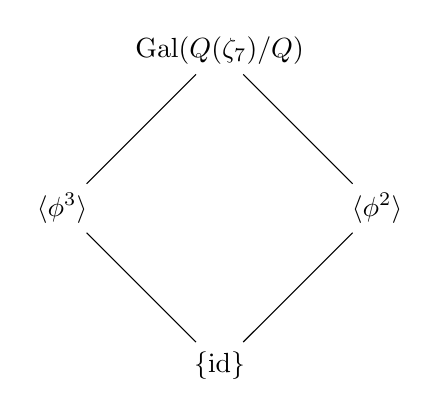
\begin{tikzpicture}[
				observed/.style = {rectangle, thick, text centered, draw, text width = 6em},
				latent/.style = {ellipse, thick, draw, text centered, text width = 6em},
				error/.style ={circle, thick, draw, text centered},
				confounding/.style = {rectangle, thick, text centered, draw, text width = 6em, minimum width = 5.5in},
				outcome/.style = {rectangle, thick, draw, text centered, minimum height = 3.5in, text width = 6em},
			]
			\node(TT) at (0,0){\(\mathrm{Gal}(\mathbb{Q}(\zeta_{7})/\mathbb{Q})\)};
			\node(TR) at (-2,-2){\(\langle \phi^{3} \rangle\)};
			\node(CR) at (2,-2){\(\langle \phi^{2} \rangle\)};
			\node(BB) at (0,-4){\(\{\mathrm{id}\}\)};

			\draw[-](BB)--(CR);
			\draw[-](BB)--(TR);
			\draw[-](CR)--(TT);
			\draw[-](TR)--(TT);
		\end{tikzpicture}
	\end{center}
	O segundo grupo é determinado por \(G = \langle \phi^{2} \rangle,\) que tem ordem 3 e forma \(G = \{\mathrm{id}, \phi^{2}, \phi^{4}\}\).

	Agora, queremos encontrar \(\mathrm{Inv}(\langle \phi^{3} \rangle)=\mathrm{Inv}(H)\); com efeito, note que \(\phi(\zeta )=\zeta^{3}\) e que (checar)
	\[
		\phi^{3}(\zeta ) = \mathrm{exp}\biggl(\frac{2\pi i}{7}6\biggr) = \mathrm{exp}\biggl(-\frac{2\pi i}{7}\biggr) = \overline{\mathrm{exp}\biggl(\frac{2\pi i}{7}\biggr)},
	\]
	e então \(\eta \coloneqq \zeta + \overline{\zeta }\) é invariante em relação a H: \(\phi^{3}(\eta ) = \eta \). Logo, \(\eta =\zeta +\overline{\zeta }\) faz parte dos elementos invariantes de H, levando à conclusão de que \(\mathbb{Q}\subsetneq \mathbb{Q}[\zeta +\overline{\zeta } ] \subseteq \mathrm{Inv}(H)\). Na verdade,
	\[
		\mathbb{Q}[\zeta +\overline{\zeta }]=\mathrm{Inv}(H);
	\]
	para demonstrar, é suficiente checar os graus. Sabemos que \(\langle \phi^{3} \rangle \trianglelefteq \mathrm{Gal}(\mathbb{Q}(\zeta_{7})/\mathbb{Q})\), tal que \(\mathrm{Inv}(H)/\mathbb{Q}\) é normal; além disso, pelo Teorema Fundamental da teoria de Galois,
	\[
		\mathrm{Gal}(\mathrm{Inv}(H)/\mathbb{Q})\cong \frac{\mathrm{Gal}(\mathbb{Q}(\zeta_7)/\mathbb{Q})}{H}.
	\]
	Porém, \(\mathrm{Gal}(\mathbb{Q}(\zeta_7)/\mathbb{Q}) = \langle \phi  \rangle\), tal que
	\[
		\mathrm{Gal}(\mathrm{Inv}(H)/\mathbb{Q})\cong \frac{\langle \phi  \rangle}{H} = \frac{\langle \phi  \rangle}{\langle \phi^{3} \rangle},
	\]
	e segue que \(\mathrm{ord}(\mathrm{Gal}(\mathrm{Inv}(H)/\mathbb{Q}))=3\). Podemos confirmar que o grau da extensão de \(\mathrm{Inv}(H)\) sobre \(\mathbb{Q}\) é 3? Sim!
	Sendo \(\mathrm{Inv}(H)/\mathbb{Q}\) Galois, então \(\mathrm{Inv}(H)\) é um corpo de decomposição de um polinômio separável, e por isso temos
	\[
		[\mathrm{Inv}(H):\mathbb{Q}] = \mathrm{ord}(\mathrm{Gal}(\mathrm{Inv}(H)/\mathbb{Q})).
	\]

	Qual é o polinômio minimal de \(\eta = \zeta +\overline{\zeta }\) sobre \(\mathbb{Q}\)? Podemos obtê-lo ao encontrar todas as raízes e aplicando à \(\eta \) todos os elementos do grupo de Galois da extensão \(\mathrm{Inv}(H)/\mathbb{Q}\)! O grupo em si é:
	\[
		\frac{\langle \phi  \rangle}{\langle \phi^{3} \rangle} = \{[\mathrm{id}], [\phi ], [\phi^{2}]\}, \quad [\mathrm{id}]=\{\mathrm{id}, \phi^{3}\},\; [\phi^{2}]=\{\phi^{2}, \phi^{5}\},\; [\phi ]=\{\mathrm{id}, \phi^{4}\}.
	\]
	Como \(\mathrm{Gal}(\mathrm{Inv}(H)/\mathbb{Q})\) age sobre \(\mathrm{Inv}(H)\), ele age também sobre \(\eta = \zeta +\overline{\zeta }\), e por isso é preciso definir a ação de \(\langle \phi  \rangle/ \langle \phi^{3} \rangle\) sobre \(\eta \); de fato, para cada \(k=0, 1, 2\), colocamos
	\[
		[\phi^{k}]\eta  \coloneqq \phi^{k}(\eta ),
	\]
	sendo necessário checar se está bem definida, por exemplo:
	\[
		[\phi^{0}=\mathrm{id}]\eta =[\phi^{3}]\eta.
	\]
	O restante é exercício.

	Logo, as raízes do polinômio minimal de \(\eta = \zeta + \overline{\zeta }\) serão
	\begin{align*}
		 & \alpha_1 \coloneqq \zeta +\zeta^{-1} ( = [\mathrm{id}]\eta ) \\
		 & \alpha_2 \coloneqq [\phi ]\eta  = \zeta^{3} + \zeta^{-3}     \\
		 & \alpha_3 \coloneqq [\phi^{2}]\eta =\zeta^{2} + \zeta^{-2},
	\end{align*}
	e construímos o polinômio com
	\[
		p(x) = (x-\alpha_1)(x-\alpha_2)(x-\alpha_3) = x^{3} + x^{2} - 2x - 1.
	\]
\end{example}
\begin{exr}
	Cheque que \(\phi^{6} = \mathrm{id}\).
\end{exr}
\begin{exr}
	Cheque que
	\[
		[\phi ]\eta =[\phi^{4}]\eta \quad\&\quad [\phi^{2}]\eta =[\phi^{5}]\eta.
	\]
\end{exr}
\begin{exr}
	Para
	\[
		G = \langle \phi^{2} \rangle\trianglelefteq \mathrm{Gal}(\mathbb{Q}(\zeta_{7})/\mathbb{Q}),
	\]
	encontre \(\mathrm{Inv}(G)\) e estude \(\mathrm{Inv}(G)/\mathbb{Q}\).
\end{exr}
\end{document}
